\documentclass[12pt,a4paper]{article}

% ── Packages ──────────────────────────────────────────────────────────────────
\usepackage[utf8]{inputenc}
\usepackage[T1]{fontenc}
\usepackage{amsmath,amssymb}
\usepackage{booktabs}
\usepackage{graphicx}
\usepackage{hyperref}
\usepackage{listings}
\usepackage{xcolor}
\usepackage{geometry}
\usepackage{caption}
\usepackage{microtype}
\usepackage{parskip}
\usepackage{lineno}

\geometry{margin=2.5cm}

\hypersetup{
  colorlinks=true,
  linkcolor=blue,
  urlcolor=blue,
  citecolor=blue
}

% ── Code listing style ────────────────────────────────────────────────────────
\lstdefinestyle{pycode}{
  language=Python,
  basicstyle=\ttfamily\small,
  keywordstyle=\color{blue}\bfseries,
  commentstyle=\color{gray},
  stringstyle=\color{teal},
  showstringspaces=false,
  breaklines=true,
  frame=single,
  framesep=4pt,
  xleftmargin=8pt,
  xrightmargin=4pt,
  numbers=none
}

% ── Title block ───────────────────────────────────────────────────────────────
\title{\textbf{pynasonde v2.0.0: Multi-Instrument Ionosonde Data Ingestion and
Automated Scaling in an Open-Source Python Library}}

\author{S. Chakraborty$^{a,*}$, T. Bullett$^{b}$, A. Barjatya$^{a}$, J. Mabie$^{b}$\\[4pt]
\small\textit{$^{a}$Embry-Riddle Aeronautical University, Daytona Beach, FL, USA}\\
\small\textit{$^{b}$Fourth State Communications, Cheyenne, WY, USA}\\[4pt]
\small$^{*}$Corresponding author. \texttt{chakras4@erau.edu}}

\date{}

% ══════════════════════════════════════════════════════════════════════════════
\begin{document}
\linenumbers
\maketitle

% ── Code Metadata ─────────────────────────────────────────────────────────────
\section*{Code metadata}
\begin{table}[h!]
\centering
\begin{tabular}{@{}lp{5.2cm}p{6.8cm}@{}}
\toprule
\textbf{Nr.} & \textbf{Code metadata description} & \textbf{Metadata} \\
\midrule
C1 & Current code version & v2.0.0 \\
C2 & Permanent link to code/repository used for this code version & \url{https://github.com/shibaji7/pynasonde} \\
C3 & Permanent link to Reproducible Capsule & \url{https://github.com/shibaji7/pynasonde} \\
C4 & Legal Code License & MIT \\
C5 & Code versioning system used & Git 2.34.1 \\
C6 & Software code languages, tools, and services used & Python 3.11 \\
C7 & Compilation requirements, operating environments \& dependencies & All dependencies are listed under Documentation \\
C8 & If available, link to developer documentation/manual & \url{https://pynasonde.readthedocs.io/en/latest/} \\
C9 & Support email for questions & chakras4@erau.edu \\
\bottomrule
\end{tabular}
\end{table}

% ── Abstract ──────────────────────────────────────────────────────────────────
\begin{abstract}
The first release of \texttt{pynasonde}~\cite{Chakraborty2026} consolidated
reading, plotting, and semi-autonomous scaling of Digisonde and Vertical
Incidence Pulsed Ionospheric Radar (VIPIR) datasets into a single open-source
Python framework, lowering the barrier to precision ionospheric analysis for
space weather forecasting, radio communication, and ionospheric research.
Since that release, two limitations became apparent in practice: several
Digisonde-family file formats in active use by collaborating stations ---
notably those produced by the Canadian Advanced Digital Ionosonde (CADI), and
the \texttt{GRM} archive format distributed by the Global Ionospheric Radio
Observatory (GIRO) \texttt{DIDBase} --- had no reading or plotting path, and
the automatic ionogram-scaling routine, effective for VIPIR, did not
generalise across the Digisonde family of raw sounding formats (\texttt{RSF},
\texttt{SBF}, \texttt{MMM}). This paper presents \texttt{pynasonde}~v2.0.0,
which closes both gaps. On the Digisonde side, the library now reads and
plots \texttt{GRM}, \texttt{RSF}, and \texttt{MMM} ionograms, connects
directly to the GIRO \texttt{DIDBase} archive, adds native support for CADI
interferometric soundings, and applies a single autoscaling routine across
the \texttt{RSF}/\texttt{SBF}/\texttt{MMM}/CADI family of echo tables. On the
VIPIR side, a seven-parameter Dynasonde-style echo extractor, an automated
URSI/CCIR ionogram scaler, and an O/X wave-mode polarization classifier now
operate directly on raw in-phase/quadrature data. Several additional
analysis modules --- true-height inversion, spread-F and irregularity
characterisation, and high-resolution sporadic-E imaging --- already exist in
the codebase and are noted as ongoing extensions toward a subsequent release,
but are not reported as delivered features here. The test suite has grown to
45 modules with continuous-integration coverage tracking, and this paper
concludes with an updated roadmap for future development.
\end{abstract}

\textbf{Keywords:} Radio wave; Ionosonde; VIPIR; CADI; Space weather; Python; Ionosphere

% ── 1. Motivation and significance ────────────────────────────────────────────
\section{Motivation and significance}
\label{sec:motivation}

The ionosphere is a magnetized, electrically charged region of the upper
atmosphere whose dynamics are driven by both terrestrial and extraterrestrial
processes~\cite{Chakraborty2026}. These drivers generate multi-scale
variability that affects high-frequency (HF) radio propagation, satellite
communication and navigation systems, and other critical infrastructure.
Vertical incidence sounders, such as Digisonde and VIPIR, play a pivotal role
in diagnosing this variability, and the first release of
\texttt{pynasonde}~\cite{Chakraborty2026} consolidated reading, plotting, and
semi-autonomous scaling of these two instrument families into a unified,
open-source Python framework.

That release, however, left two classes of gap. First, several file formats
produced by collaborating stations had no parser or plotting path at all: the
Canadian Advanced Digital Ionosonde (CADI), a community-maintained instrument
widely deployed at mid- and high-latitude stations, and the \texttt{GRM}
archive format --- a raw concatenation of \texttt{RSF}/\texttt{SBF}/\texttt{MMM}
blocks distributed by the University of Massachusetts Lowell's Global
Ionospheric Radio Observatory (GIRO) \texttt{DIDBase}~\cite{ReinischGalkin2011}
--- for which \texttt{pynasonde} v1.0.0 also had no remote-access connector.
Second, the automated ionogram-scaling routine introduced in v1.0.0 was
implemented only for VIPIR vertical ionograms; it did not extend to the raw
Digisonde sounding formats (\texttt{RSF}, \texttt{SBF}, \texttt{MMM}), so
stations without VIPIR hardware could not benefit from automated parameter
extraction. This paper describes \texttt{pynasonde}~v2.0.0, which closes both
gaps: new reading and plotting support for \texttt{GRM}, \texttt{MMM}, and
CADI data; a read connector to the \texttt{DIDBase} archive; a single
autoscaling routine spanning the \texttt{RSF}/\texttt{SBF}/\texttt{MMM}/CADI
family; and, on the VIPIR side, a seven-parameter echo extractor, an
automated URSI/CCIR scaler, and an O/X polarization classifier operating
directly on raw in-phase/quadrature (I/Q) data.

\paragraph{New instrument and archive access in v2.} The Digisonde and VIPIR
instrument families were introduced in the original
release~\cite{Chakraborty2026}. Version 2.0.0 adds native support for the
Canadian Advanced Digital Ionosonde (CADI), a digital ionosonde used at a
number of community-operated stations and distributed independently of the
Digisonde DPS4D line. CADI records amplitude and phase at multiple receivers
per pulse in its own MD2/MD4 binary format, enabling interferometric
angle-of-arrival and O/X mode determination analogous to what the VIPIR
seven-parameter extractor (Section~\ref{ssec:functionalities}) provides for
RIQ data. Version 2.0.0 also adds a read-only connector to GIRO
\texttt{DIDBase}~\cite{ReinischGalkin2011}, the University of Massachusetts
Lowell's community archive of Digisonde data, allowing stations and
collaborators to pull raw ionogram files or parsed DataFrames directly from
the archive rather than only from locally held files.

% ── 2. Software description ───────────────────────────────────────────────────
\section{Software description}
\label{sec:software}

The primary objective of \texttt{pynasonde} remains to provide tools for
reading, visualising, and semi-autonomously processing ionosonde datasets,
extracting scaled parameters from ionograms. Version 2.0.0 extends this
objective in two directions: it broadens the set of file formats and
instruments that can be read and plotted, and it extends automated scaling
from VIPIR alone to the full family of Digisonde and CADI raw sounding
formats.

\subsection{Software architecture}
\label{ssec:architecture}

The library remains organised into two primary modules, \texttt{digisonde}
and \texttt{vipir}, each dedicated to the corresponding instrument family.
Table~\ref{tab:formats} summarises the file formats now supported and marks
those newly added or repaired in v2.0.0 relative to the v1.0.0
release~\cite{Chakraborty2026}. Within \texttt{digisonde}, the \texttt{RSF}
and \texttt{SBF} parsers were also refactored onto a shared binary-block
base class, removing several hundred lines of duplicated decoding logic that
had accumulated as the two formats evolved independently.

\begin{table}[h!]
\caption{Description of primary data file formats supported by
\texttt{pynasonde} v2.0.0. Formats marked \emph{(new)} were not readable in
v1.0.0.}
\label{tab:formats}
\centering
\begin{tabular}{@{}llp{6.3cm}@{}}
\toprule
\textbf{Extension} & \textbf{Type} & \textbf{Source instrument / Description} \\
\midrule
RSF        & Binary & Digisonde --- complete sounding information \\
SBF        & Binary & Digisonde --- complete sounding information \\
SAO 4.3    & ASCII  & Digisonde --- ARTIST scaled data with echo traces \\
SAO 5.0    & XML    & Digisonde --- ARTIST scaled data with echo traces; multi-record day-files \emph{(new)} \\
DFT        & ASCII  & Digisonde --- Doppler spectra per sounding frequency \\
DVL        & ASCII  & Digisonde --- derived Doppler velocity \\
SKY        & ASCII  & Digisonde --- Doppler information from individual echoes \\
EDP        & ASCII  & Digisonde --- electron density profile \emph{(repaired; v1.0.0 loader silently returned no data)} \\
MMM        & Binary & Digisonde --- ModMax max-Doppler-channel amplitude ionogram \emph{(new)} \\
GRM        & Binary & Digisonde archive --- concatenated RSF/SBF/MMM blocks from GIRO DIDBase; auto-detected and split \emph{(new)} \\
MD2/MD4    & Binary & CADI --- interferometric raw soundings; amplitude, phase, cross-receiver baselines \emph{(new)} \\
RIQ        & Binary & VIPIR --- raw I/Q data \\
NGI/SDR    & Binary & VIPIR --- NetCDF processed ionograms \\
\bottomrule
\end{tabular}
\end{table}

Within \texttt{digisonde}, the new \texttt{GrmSplitter} auto-detects the
record type embedded in a \texttt{GRM} archive (RSF~$=$~7, SBF~$=$~3,
MMM~$=$~9) directly from the byte stream, and either splits the archive to
individual files or lazily loads each embedded ionogram in parallel, handing
each one to the plotting routine appropriate for its underlying format. The
new \texttt{CadiExtractor} decodes the CADI MD2/MD4 binary format into raw
and product-level DataFrames, the latter carrying per-echo amplitude, phase,
cross-receiver baseline phase differences, and coherence. The new
\texttt{DidBaseConnector} connects to GIRO \texttt{DIDBase} over its Firebird
SQL interface, listing available stations and fetching raw files or parsed
DataFrames for a station and date range in any supported format. Finally, the
\texttt{digisonde.scaler} package generalises the scaling routine introduced
in v1.0.0: a schema-detection layer normalises RSF/SBF, MMM, or CADI echo
columns onto one canonical table, after which the same clustering,
RFI-filtering, and layer-height estimation logic runs unchanged regardless of
which format produced the input.

Within \texttt{vipir}, the new \texttt{EchoExtractor} implements
Dynasonde-style seven-parameter echo extraction~\cite{Zabotin2005} directly
from RIQ in-phase/quadrature cubes, in place of the coarser, image-based
scaling that v1.0.0 applied only to already-processed SDR ionograms. Building
on its output, the new \texttt{IonogramScaler} derives standard URSI/CCIR
parameters, and the new \texttt{PolarizationClassifier} labels each echo as
O-, X-mode, or ambiguous.

\subsection{Software functionalities}
\label{ssec:functionalities}

The functionalities introduced in v1.0.0 --- generic and instrument-specific
plotting routines, and the image-segmentation-based \texttt{scale()} method
for VIPIR ionograms~\cite{Chakraborty2026} --- are unchanged in v2.0.0. This
section describes the working principles of the new v2.0.0 functionality.
Section~\ref{sec:examples} provides illustrative examples and figures for
each.

\subsubsection{Working principle of GRM/MMM plotting and CADI extraction}

A \texttt{GRM} archive downloaded from \texttt{DIDBase} is a raw
concatenation of 4096-byte \texttt{RSF}/\texttt{SBF}/\texttt{MMM} blocks with
no separating structure other than a one-byte record-type tag at the start
of each block. \texttt{GrmSplitter} performs a single sequential scan to
record the byte offset, length, and record type of every embedded ionogram,
then dispatches parallel workers to extract each one, so that splitting or
loading a multi-gigabyte archive does not require holding it in memory at
once. Each recovered \texttt{MMM} ionogram is binned onto a regular
frequency--height grid and rendered as a pcolormesh image, taking the
maximum amplitude across Doppler channels per cell (the ``brightest echo''
convention used by SAOExplorer), with combined O$+$X and side-by-side O/X
views. CADI MD2/MD4 files are decoded block-by-block into per-receiver
amplitude and phase samples; \texttt{CadiExtractor} reduces these to a
per-echo product table carrying cross-receiver baseline phase differences
and coherence, from which wave mode and angle of arrival can be estimated in
the same spirit as the VIPIR seven-parameter extractor described below.

\subsubsection{Working principle of DIDBase access and cross-format scaling}

\texttt{DidBaseConnector} opens a connection to the GIRO
\texttt{DIDBase}~\cite{ReinischGalkin2011} Firebird SQL database using the
native \texttt{fdb} Python client, requiring only a host, database role, and
credentials. It exposes a station list, a file-fetching method that
downloads raw ionogram files for a station and date range in a chosen
format, and a DataFrame-returning method that parses the fetched files
directly, without requiring an intermediate on-disk step. The
\texttt{digisonde.scaler} package that consumes this data (or any locally
held \texttt{RSF}/\texttt{SBF}/\texttt{MMM}/CADI file) is DataFrame-native
rather than format-specific: a schema-detection step recognises the
column layout of each source format and normalises it onto one canonical
echo table, after which a Viterbi-style dynamic-programming tracker follows
the strongest coherent trace across frequency, and RANSAC- and
DBSCAN-regularised post-processing~\cite{Xu2009} produces layer-height
estimates. Because the normalisation step is the only format-specific code
path, adding a new Digisonde-family format to the autoscaler in the future
requires no change to the scaling logic itself.

\subsubsection{Working principle of VIPIR echo extraction, scaling, and polarization}

For each pulse set (one sounding frequency step) in a raw RIQ file,
\texttt{EchoExtractor} builds a complex I/Q cube of shape (pulse count, gate
count, receiver count) and, for every range gate whose coherent
signal-to-noise ratio exceeds a configurable threshold, computes the seven
Dynasonde-style echo parameters~\cite{Zabotin2005}: gross phase, Doppler
velocity, stationary-phase group range, eastward and northward echo
location, polarization chirality, and planar-wavefront residual, alongside
peak amplitude. The resulting per-echo table feeds two downstream routines.
\texttt{IonogramScaler} derives the standard URSI/CCIR parameters --- foE,
h$'$E, foF1, h$'$F, foF2, h$'$F2, MUF(3000), and M(3000)F2 --- from a
filtered, mode-labelled trace, with bootstrap-resampled uncertainty on foF2
and h$'$F2. \texttt{PolarizationClassifier} labels each echo O-mode, X-mode,
or ambiguous by thresholding the sign of the polarization-chirality
parameter against a configurable convention that accounts for the local
geomagnetic hemisphere and antenna wiring, so that scaling and further
analysis can be restricted to a single, unambiguous propagation mode.

% ── 3. Illustrative examples ─────────────────────────────────────────────────
\section{Illustrative examples}
\label{sec:examples}

The \texttt{pynasonde} library continues to follow recommended community best
practices~\cite{Burrell2018} and is implemented in Python (version 3.11 or
later). Version 2.0.0 adds three dependencies to those listed in the
original release~\cite{Chakraborty2026}: \texttt{netCDF4} (a hard runtime
import that was missing from v1.0.0's declared dependencies),
\texttt{scikit-learn} (RANSAC and DBSCAN regularisation in the cross-format
scaler), and, optionally, \texttt{fdb} for \texttt{DidBaseConnector}. Table~
\ref{tab:deps} summarises the updated dependency list. Installation remains
available through PyPI (\texttt{pip install pynasonde}) or, for development,
by cloning the repository as shown in Listing~1 of the original
release~\cite{Chakraborty2026}.

\begin{table}[h!]
\caption{Version v2.0.0 library dependencies (additions since v1.0.0 in italics).}
\label{tab:deps}
\centering
\begin{tabular}{@{}ll@{}}
\toprule
\textbf{Required} & \textbf{Testing / Optional} \\
\midrule
numpy         & pytest \\
pandas        & coverage[toml] \\
matplotlib    & pytest-cov \\
opencv-python-headless & \emph{scikit-learn} \\
SciencePlots  & \emph{fdb (DIDBase, optional)} \\
timezonefinder & \\
scipy         & \\
loguru        & \\
\emph{netCDF4} & \\
\bottomrule
\end{tabular}
\end{table}

As in the original release, each example below is a step-by-step conceptual
description of an end-to-end workflow; complete executable scripts are
provided in the \texttt{examples/} directory of the GitHub repository.

\subsection{Reading and plotting GRM and MMM files}

A \texttt{GRM} archive is opened with \texttt{GrmSplitter}, which reports the
auto-detected record type and returns a combined DataFrame across every
embedded ionogram via \texttt{load\_dataframes()}. When the recovered
records are \texttt{MMM} blocks, the resulting frequency--height, Doppler
channel, and polarisation columns are binned and rendered as O/X pcolormesh
ionograms; when they are \texttt{RSF} or \texttt{SBF} blocks, the same
direction-coded ionogram and directogram routines described below apply
directly. Fig.~\ref{fig:grm} shows an application of this workflow to
archival WP937 GRM data spanning both the RSF/MMM and MMM eras of that
station's Digisonde hardware: O-mode power is binned onto a common,
256-bin-compatible virtual-height grid (5~km bins, matching the classic DPS
height-gate table) and a regular time grid, then split by frequency band,
making the diurnal persistence of the 110--140~km E/Es layer directly
comparable across soundings taken two years apart on different source
hardware.

\begin{figure}[h!]
  \centering
  \includegraphics[width=0.85\textwidth]{../../docs/examples/figures/WP937_19990705_grm_d256_compatible_power_bins.png}
  \caption{O-mode power derived from WP937 GRM-archived soundings, binned
    onto a common virtual-height/time grid and split by frequency band
    (1999-07-05).}
  \label{fig:grm}
\end{figure}

\subsection{Reading and plotting RSF direction-coded ionograms and directograms}

The example script \texttt{rsf\_direction\_ionogram.py}, provided in the
\texttt{examples/digisonde/} directory, demonstrates direction-coded
ionogram plotting and daily directogram generation from raw \texttt{RSF}
files using \texttt{RsfExtractor} and \texttt{RsfIonogram}. A single sounding
is rendered as a frequency--height ionogram colour-coded by echo arrival
direction, and a full day of soundings is stacked into a directogram (ground
distance versus UT time, amplitude-coloured) that reveals small-scale,
transient structures --- such as sporadic-E patches or travelling
disturbances --- not visible in any single ionogram. Fig.~\ref{fig:rsfdir}
shows both products for station KR835.

\begin{figure}[h!]
  \centering
  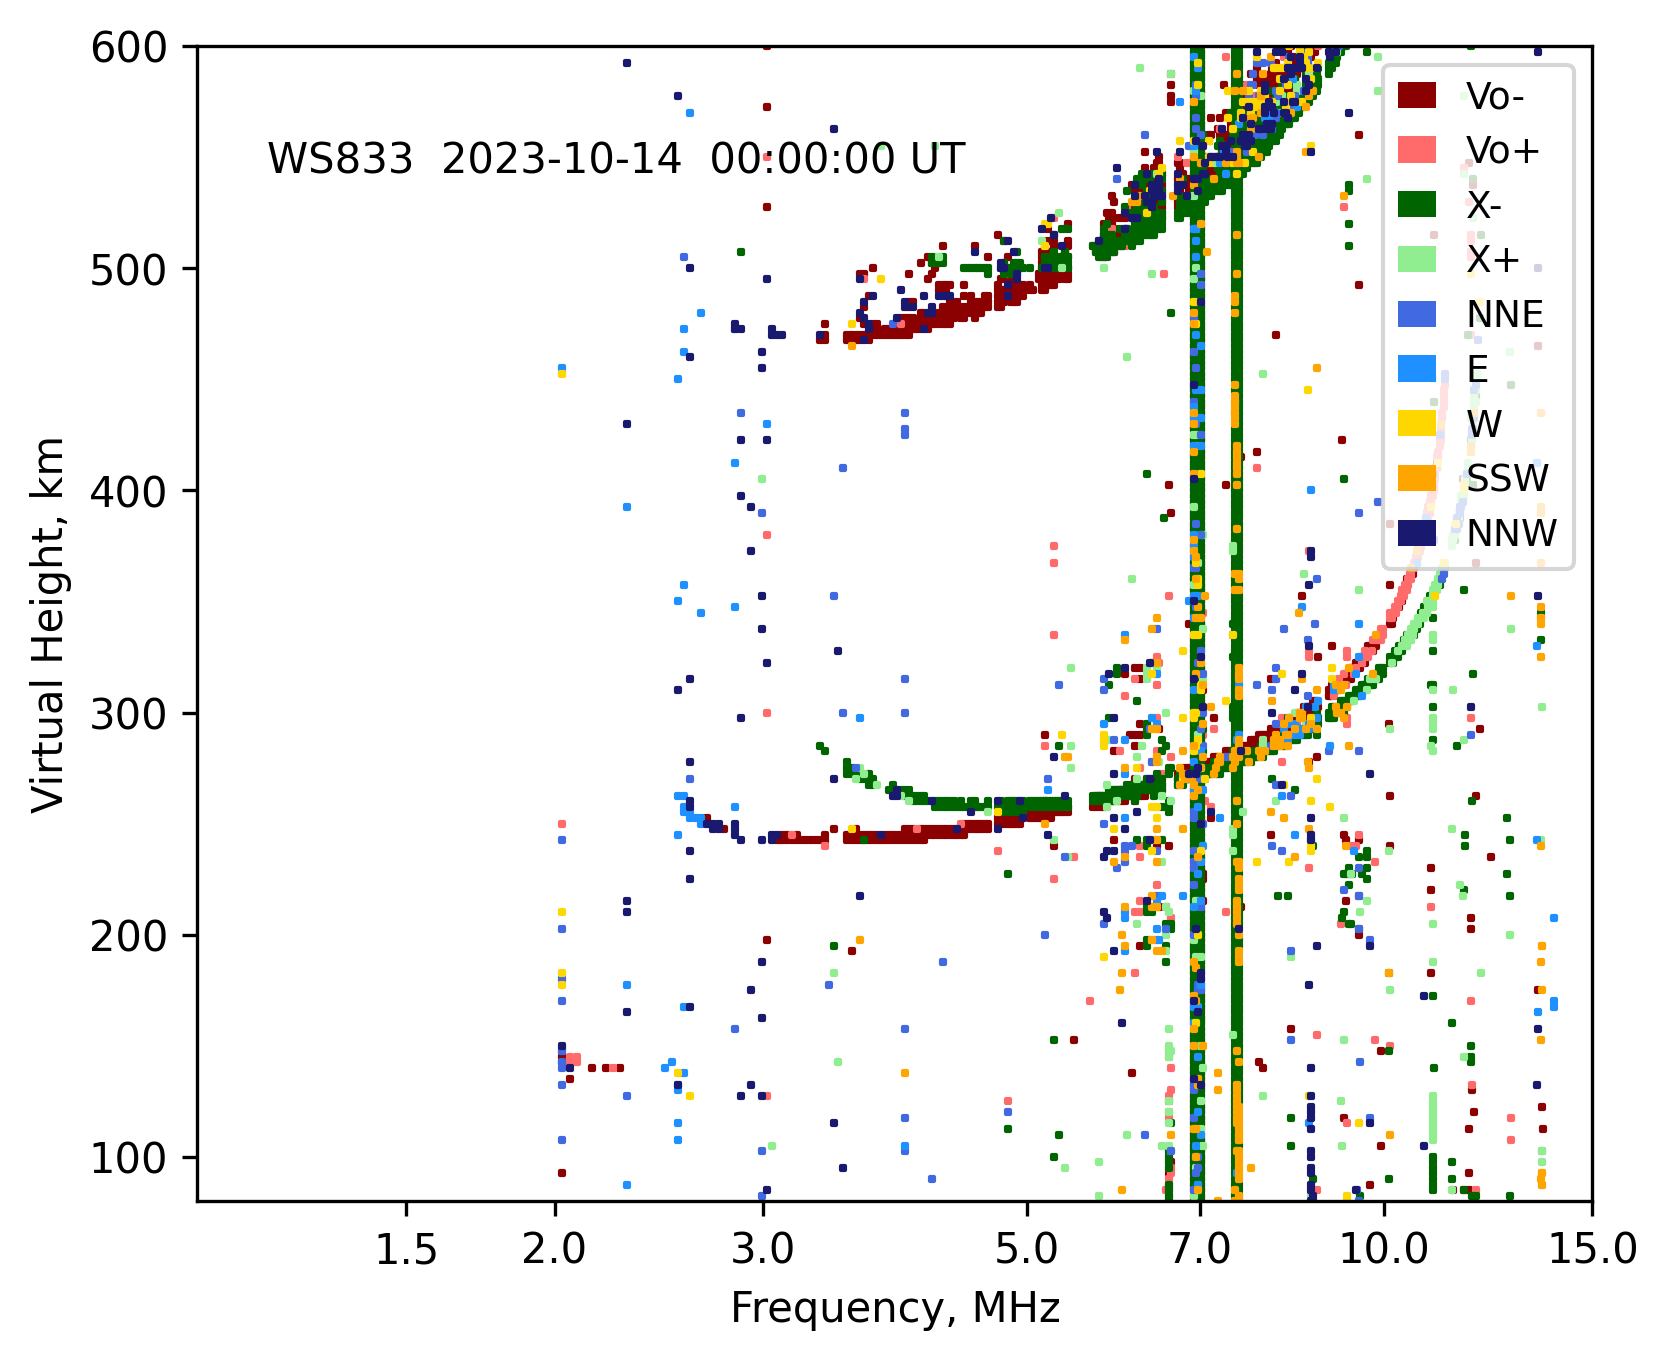
\includegraphics[width=0.47\textwidth]{../../docs/examples/figures/rsf_direction_ionogram_KR835.png}
  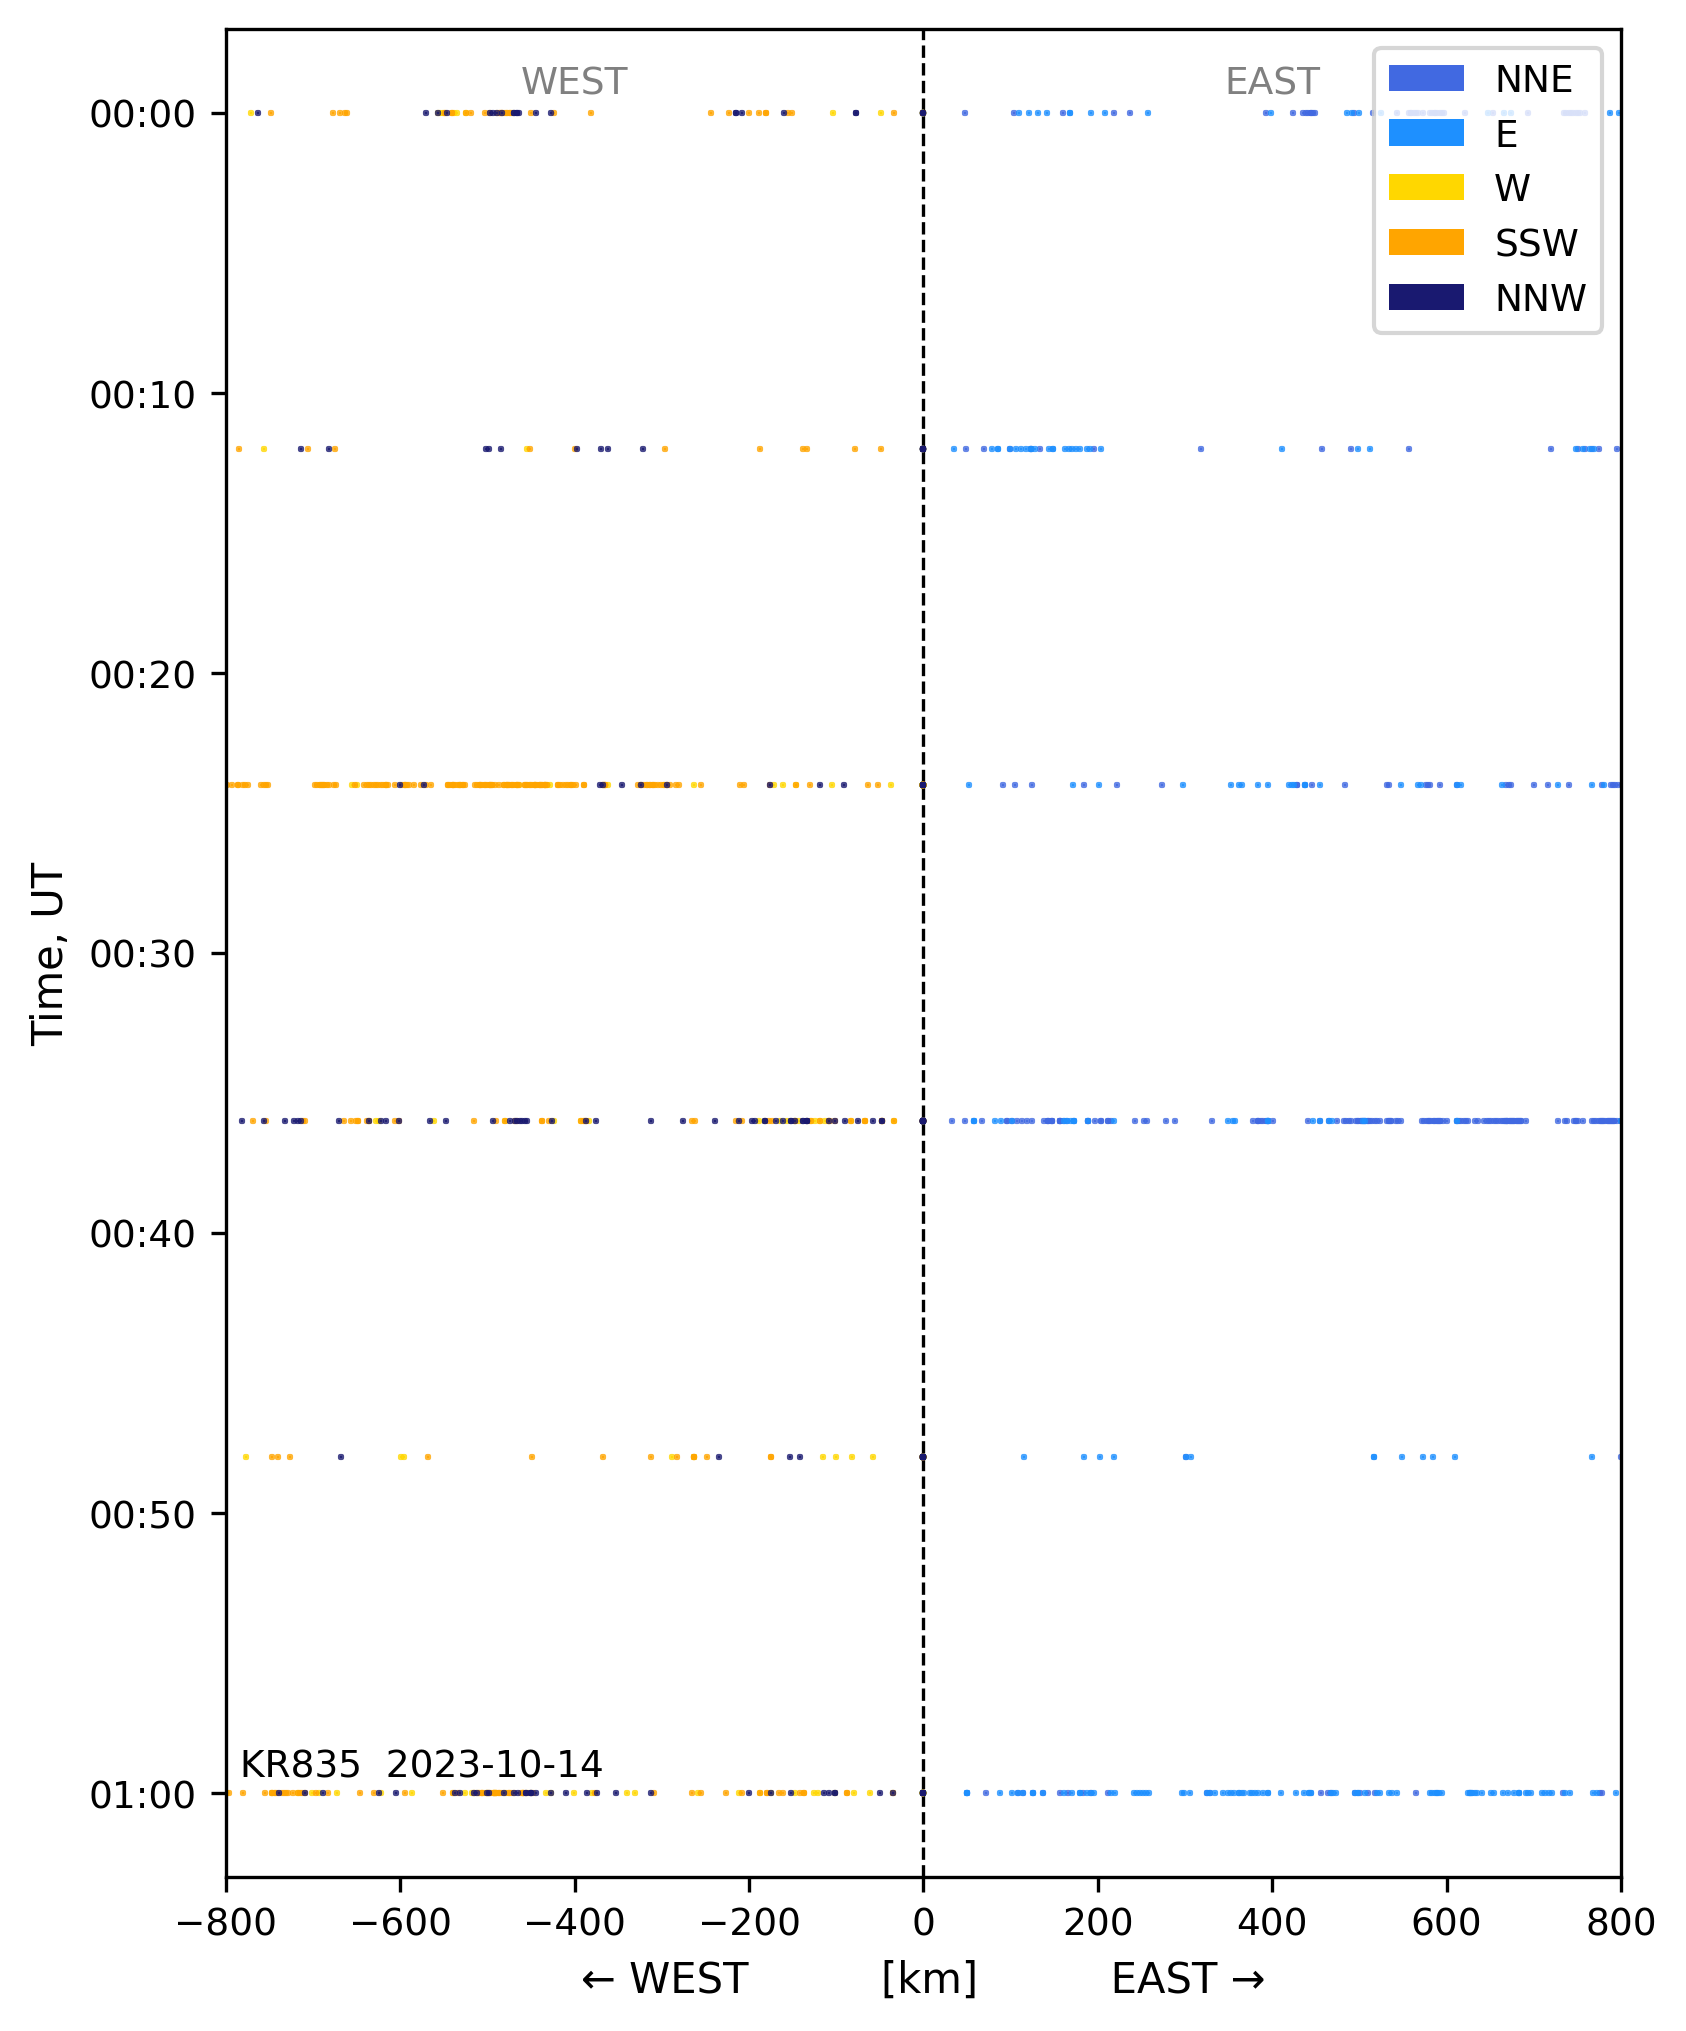
\includegraphics[width=0.47\textwidth]{../../docs/examples/figures/rsf_directogram_KR835_daily.png}
  \caption{Left: direction-coded RSF ionogram for KR835 (colour = arrival
    azimuth). Right: daily directogram for the same station (time vs.\
    ground distance, amplitude-coloured).}
  \label{fig:rsfdir}
\end{figure}

\subsection{Reading CADI files and cross-format autoscaling}

The example scripts \texttt{cadi\_products.py} and
\texttt{cadi\_interferometry\_plot.py}, provided in
\texttt{examples/digisonde/}, demonstrate loading CADI MD2/MD4 files with the
\texttt{CadiExtractor} class method \texttt{load\_CADI\_files()} (with
\texttt{product="products"} or \texttt{"echoes"}) and rendering the
resulting cross-receiver baseline phase differences as an
O/X-mode diagnostic (Fig.~\ref{fig:cadi}). The example script
\texttt{rsf\_scaler.py} demonstrates the companion cross-format autoscaler:
an \texttt{RSF} file is loaded with \texttt{RsfExtractor}, converted to a
DataFrame, and passed to \texttt{scale\_dataframe()} with
\texttt{method="viterbi"} together with per-layer height and frequency
windows; the same call, with no change to the scaling logic, accepts
\texttt{SBF}, \texttt{MMM}, or CADI product DataFrames. Fig.~\ref{fig:scaler} shows the resulting Viterbi E/F2
traces overlaid on the raw O/X ionogram.

\begin{figure}[h!]
  \centering
  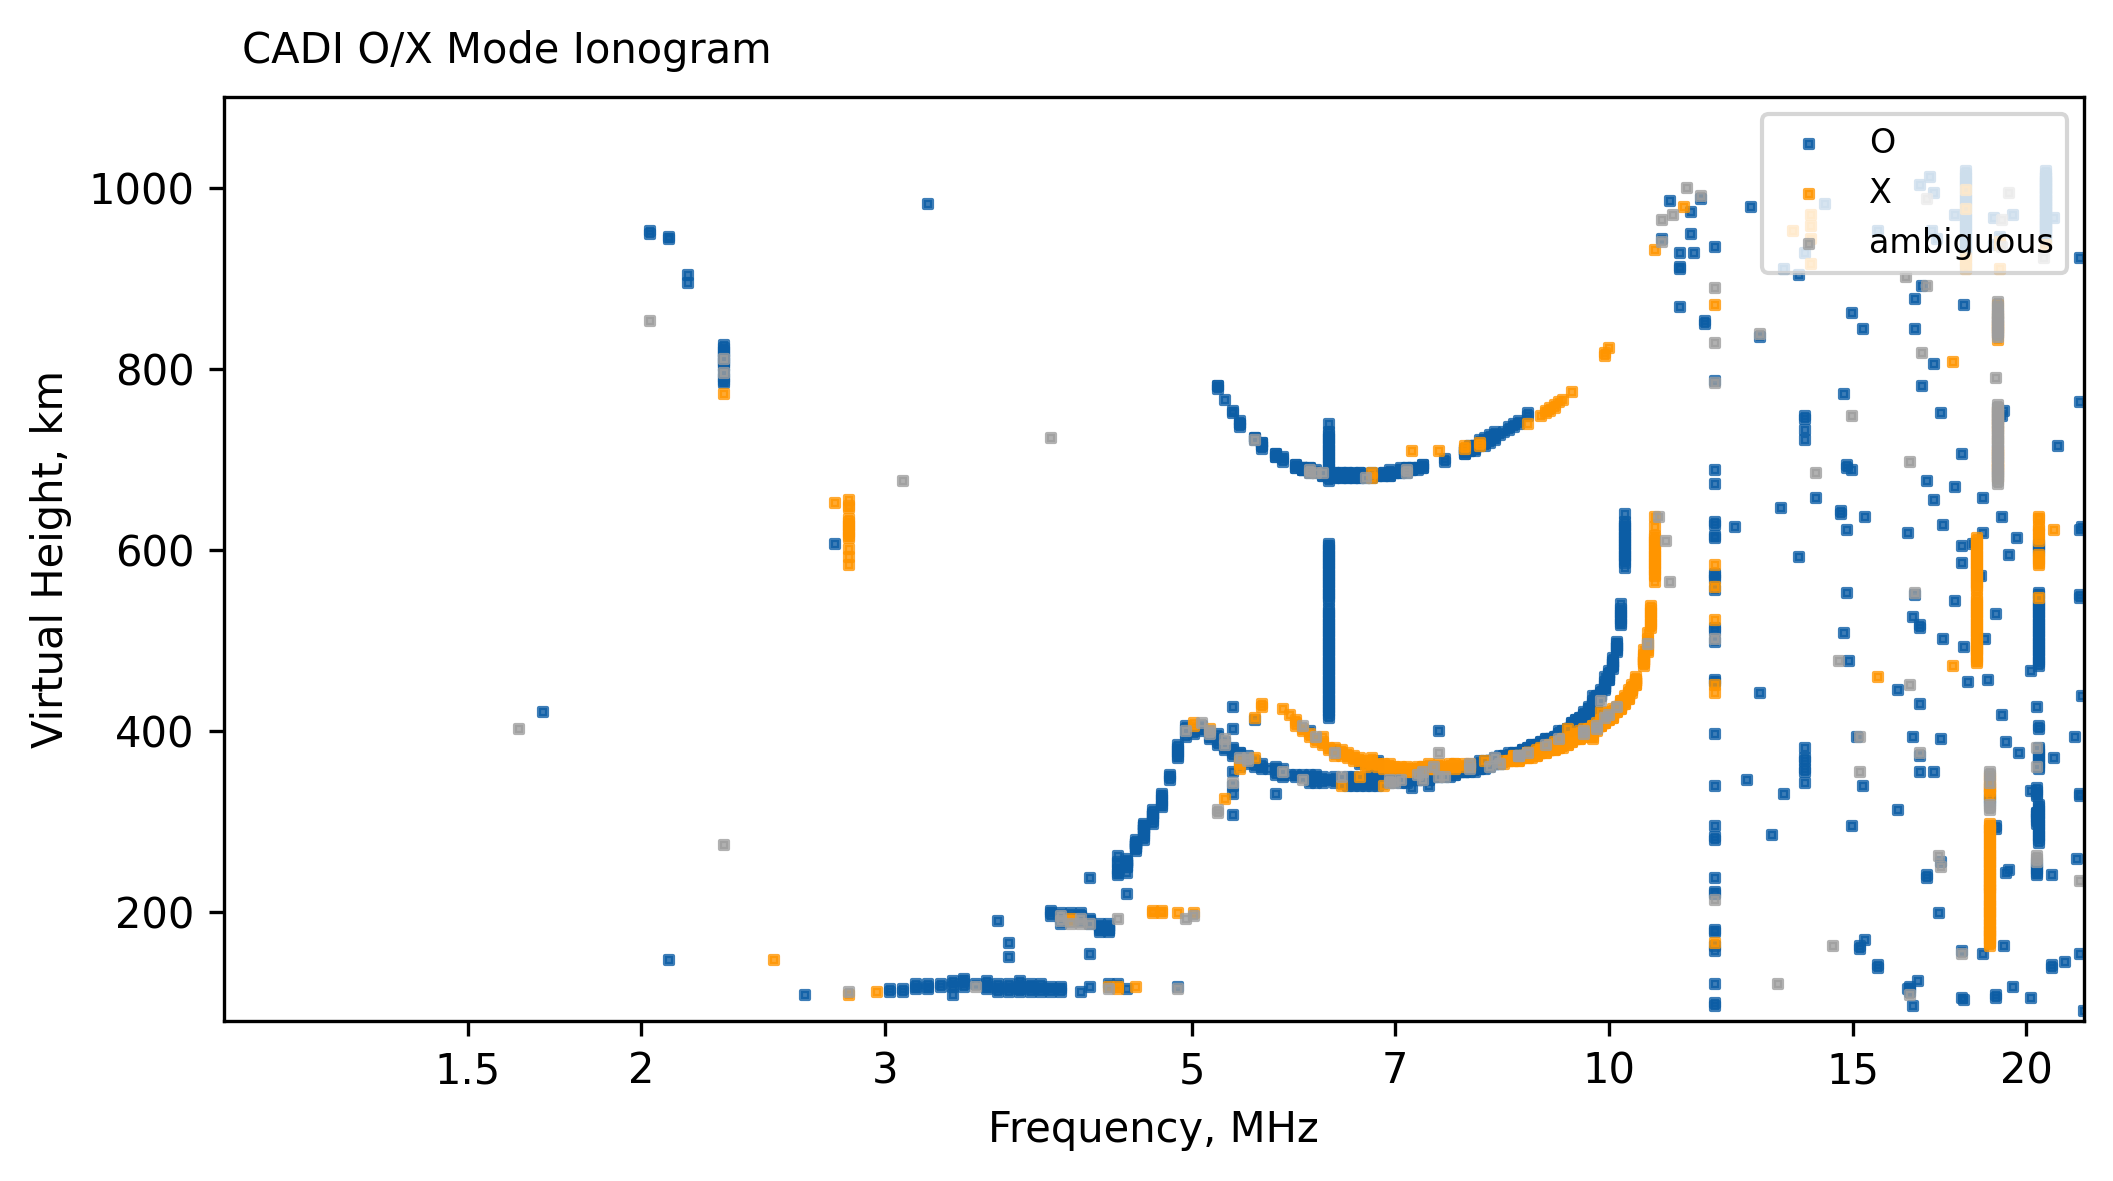
\includegraphics[width=0.55\textwidth]{../../docs/examples/figures/cadi_ox_mode_scatter.png}
  \caption{O/X-mode separation derived from CADI cross-receiver baseline
    phase differences (\texttt{CadiExtractor}, \texttt{product="echoes"}).}
  \label{fig:cadi}
\end{figure}

\begin{figure}[h!]
  \centering
  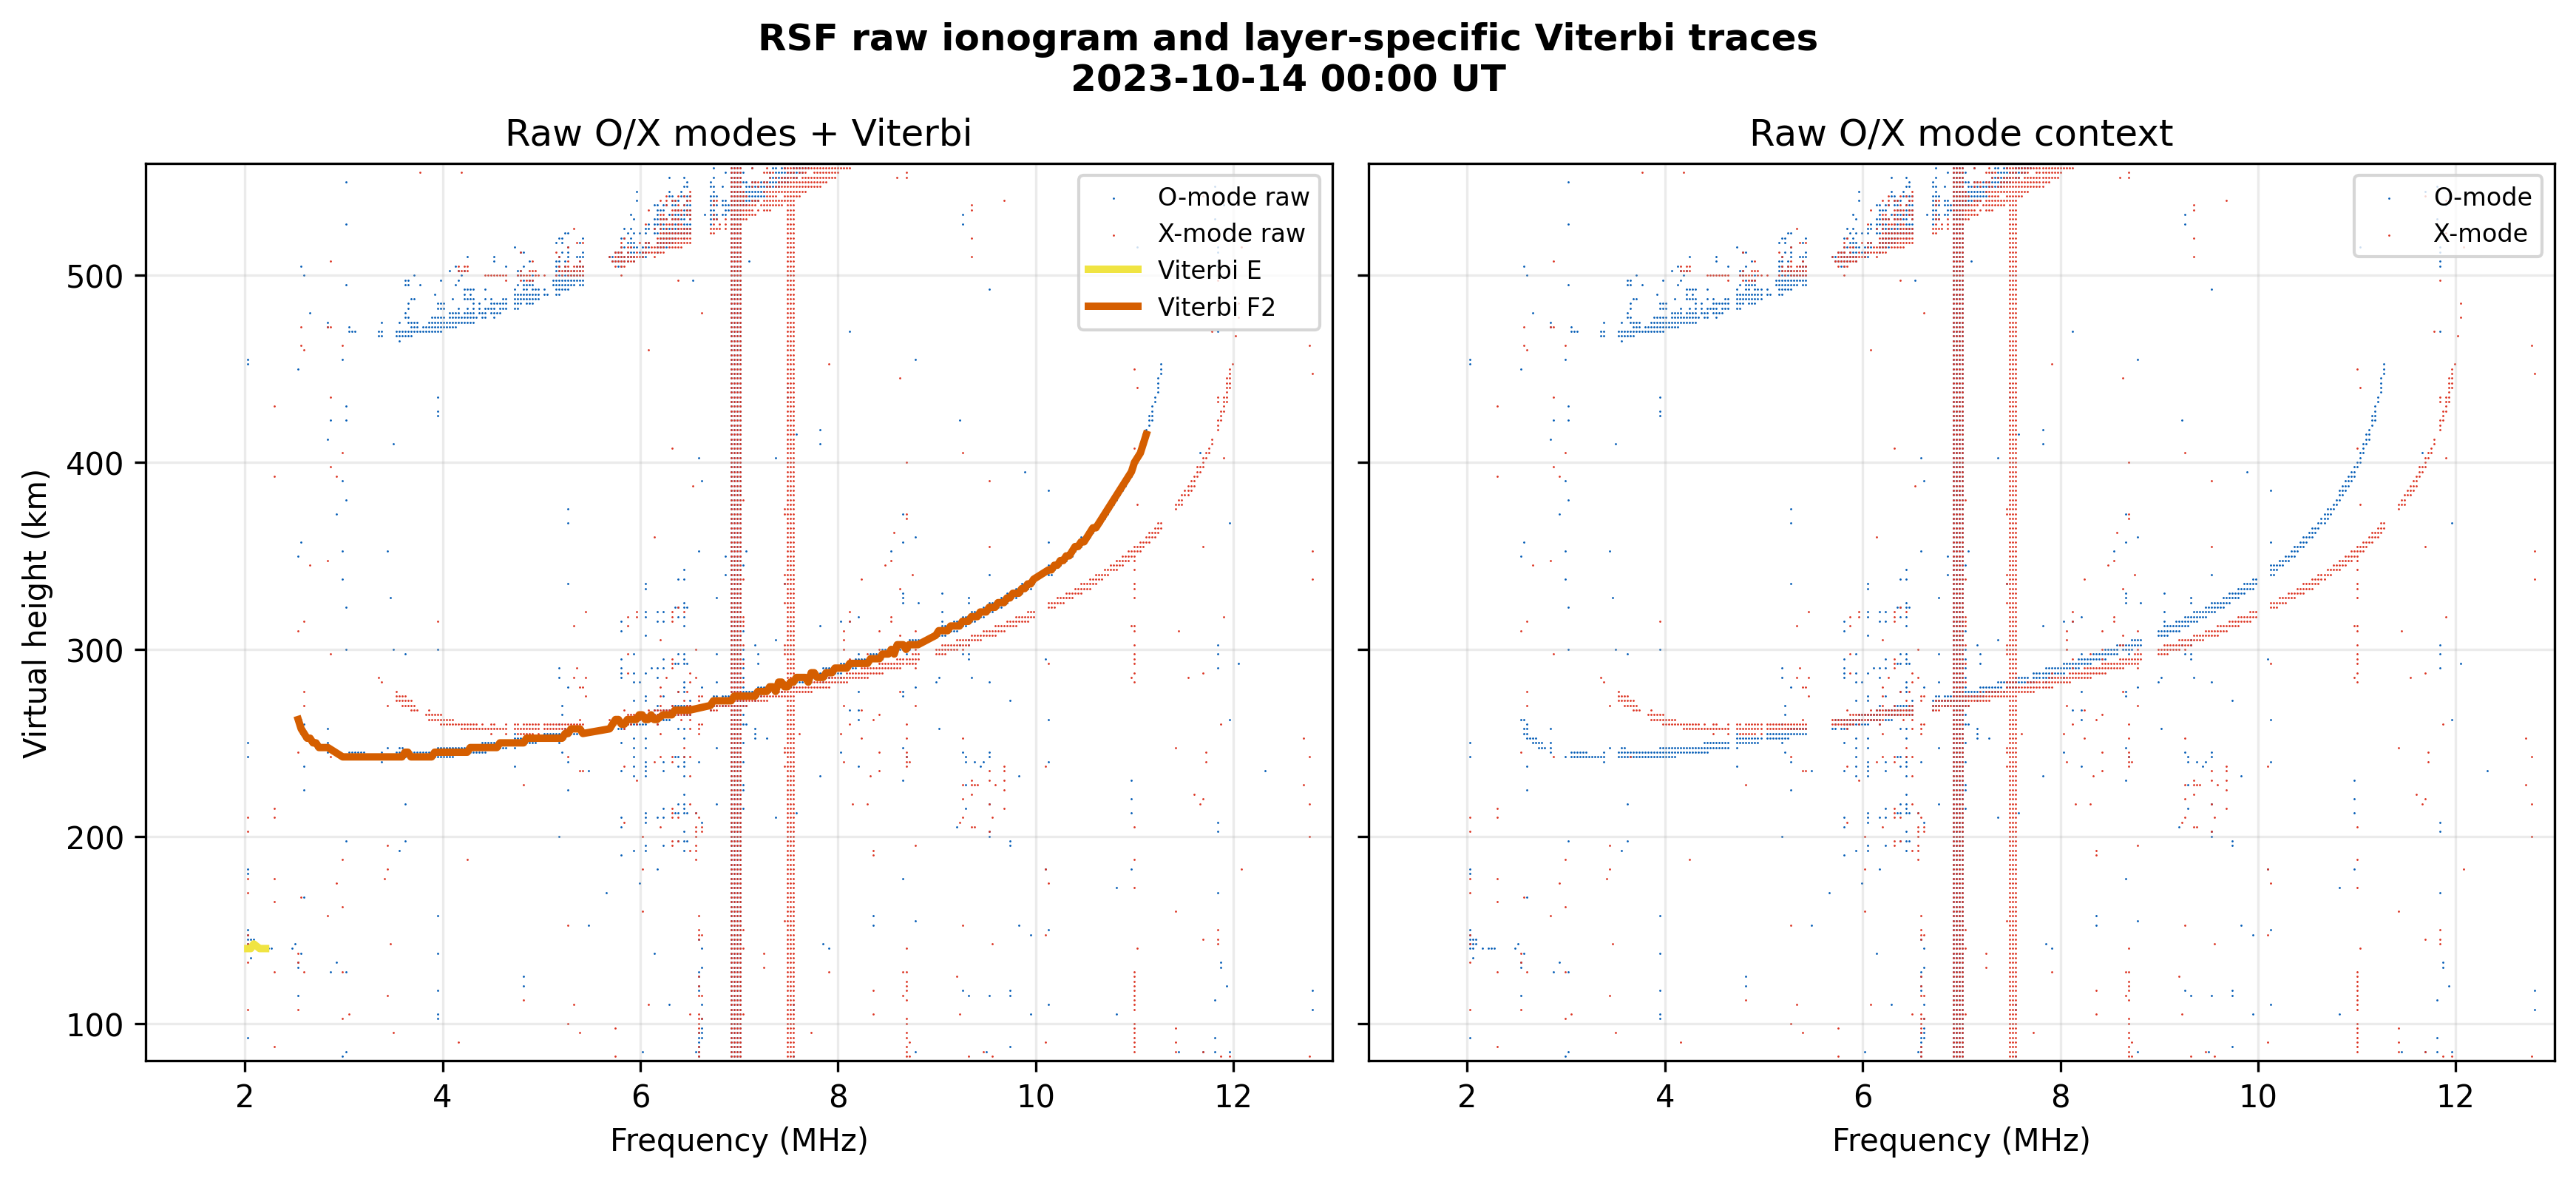
\includegraphics[width=0.8\textwidth]{../../docs/examples/figures/rsf_scaler_viterbi.png}
  \caption{Raw RSF O/X ionogram with layer-specific Viterbi traces from the
    cross-format autoscaler (\texttt{scale\_dataframe}).}
  \label{fig:scaler}
\end{figure}

\subsection{Reading RIQ datasets: echo extraction, scaling, and polarization}

Building on the \texttt{proc\_riq.py} workflow from the original
release~\cite{Chakraborty2026}, a raw \texttt{RIQ} file is now additionally
passed to \texttt{EchoExtractor}, which derives the seven Dynasonde-style
echo parameters for every coherent range gate in every pulse set and returns
a DataFrame or \texttt{xarray.Dataset}. This table is passed in turn to
\texttt{PolarizationClassifier}, which labels each echo O-, X-mode, or
ambiguous, and to \texttt{IonogramScaler}, which derives foE, foF2, h$'$F2,
and MUF(3000) from the O-mode-only subset. Fig.~\ref{fig:echo} shows the
resulting six-panel diagnostic (ionogram, direction cosines, Doppler
velocity, and polarization) for a WI937 sounding.

\begin{figure}[h!]
  \centering
  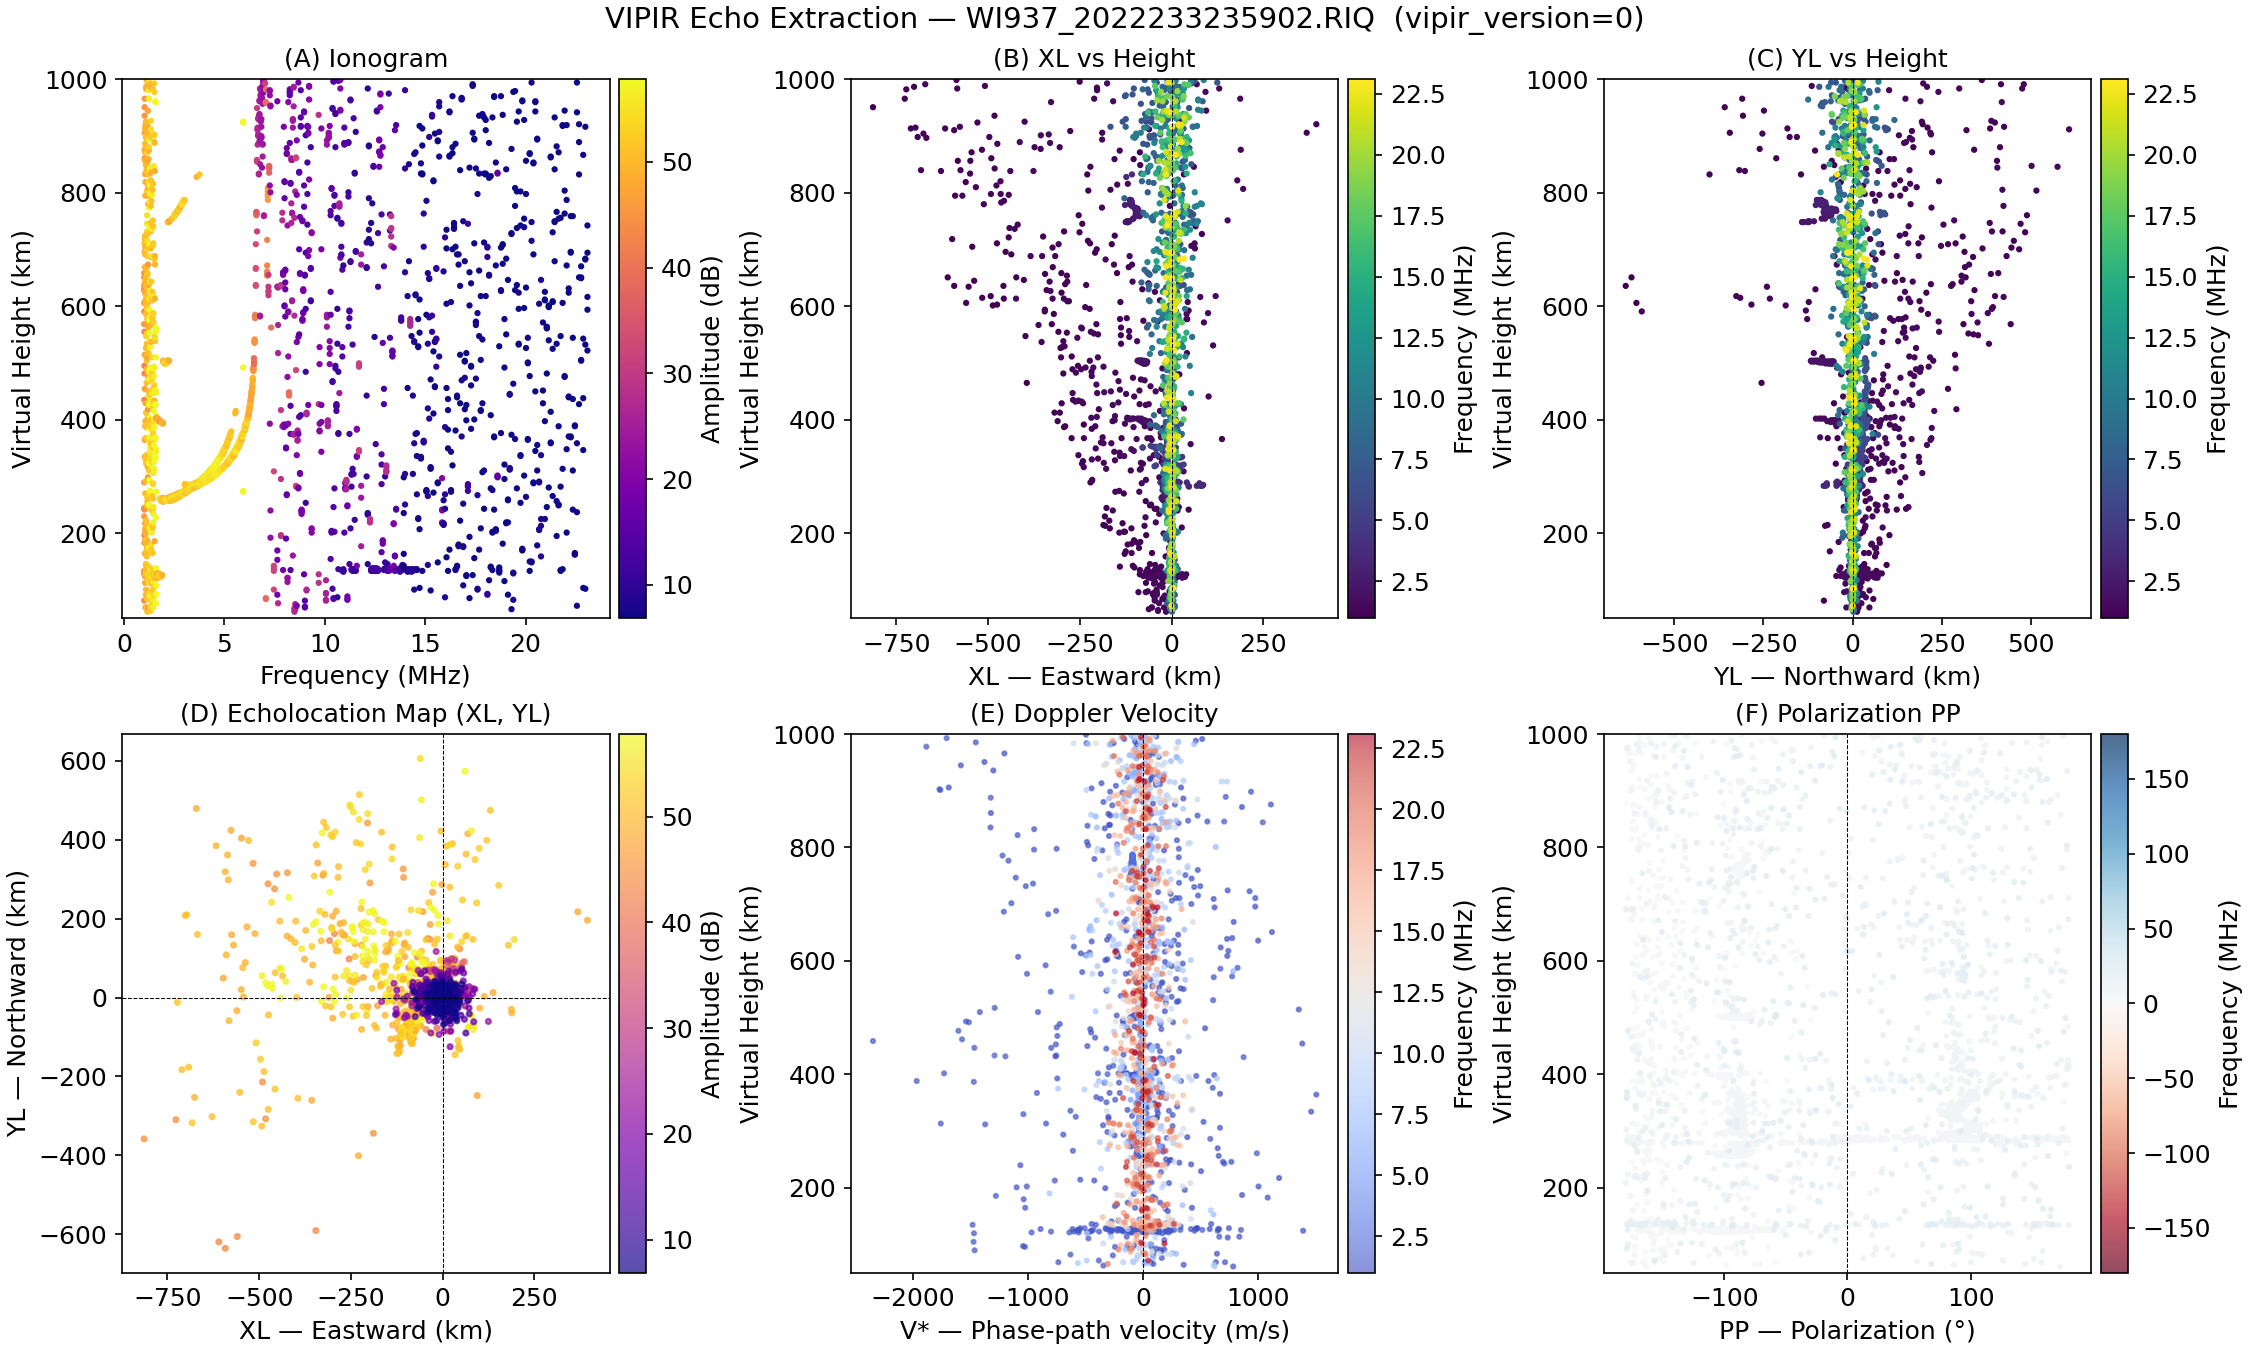
\includegraphics[width=0.75\textwidth]{../../docs/examples/figures/echo_extraction_wi937.png}
  \caption{Six-panel echo-extraction diagnostic for a WI937 RIQ sounding:
    ionogram, XL/YL direction cosines, Doppler velocity, and polarization
    (PP).}
  \label{fig:echo}
\end{figure}

% ── 4. Impact ────────────────────────────────────────────────────────────────
\section{Impact}
\label{sec:impact}

This release extends a library that already modernises and unifies tools for
reading, plotting, and analysing observations from vertical incidence MF/HF
instruments~\cite{Chakraborty2026}. Adding native CADI support extends that
reach to a widely deployed community instrument that previously required
station-specific scripts outside the \texttt{pynasonde} framework, while the
\texttt{DIDBase} connector removes the need to manually download and
re-parse community-archived files before analysis can begin. The single
autoscaling routine spanning \texttt{RSF}, \texttt{SBF}, \texttt{MMM}, and
CADI echo tables means that stations without VIPIR hardware, including many
legacy and community-operated Digisonde installations, can now benefit from
the same automated parameter extraction previously available only for VIPIR
ionograms. On the VIPIR side, the seven-parameter echo extractor, automated
URSI/CCIR scaler, and O/X polarization classifier together remove a
manual-scaling step that has historically limited the throughput of
ionosonde networks, turning raw I/Q data directly into standard ionospheric
parameters. As with the original release, these tools are expected to
support multi-point and multi-instrument space-weather studies that
integrate ground-based and space-borne observations~\cite{Chakraborty2026},
and the expanded format coverage specifically enables the inclusion of CADI-
and \texttt{DIDBase}-archived stations in such studies for the first time
within this framework.

% ── 5. Future development and conclusion ─────────────────────────────────────
\section{Future development and conclusion}
\label{sec:conclusions}

Version 2.0.0 of \texttt{pynasonde} closes the two gaps identified in
Section~\ref{sec:motivation}: missing instrument and archive coverage
(CADI, \texttt{GRM}, \texttt{MMM}, \texttt{DIDBase}), and scaling that did
not extend beyond VIPIR. Table~\ref{tab:roadmap} updates the tentative
roadmap first published with v1.0.0~\cite{Chakraborty2026}, marking items
delivered in this release and adding the items now targeted for subsequent
releases. Several analysis modules --- an Abel/lamination true-height
inversion, spread-F and small-scale irregularity characterisation from
residual-phase structure functions, and Capon high-resolution sporadic-E
cross-spectrum imaging --- already exist in the \texttt{pynasonde} codebase
on top of the VIPIR echo-extraction layer described here, but are not yet
validated to the standard of a reportable release feature and are therefore
excluded from this paper; they are expected to be documented in a future
version once validated against independent measurements.

\begin{table}[h!]
\caption{Expected functionalities associated with tentative future releases,
updated from Table 3 of the original release~\cite{Chakraborty2026}.}
\label{tab:roadmap}
\centering
\begin{tabular}{@{}lp{9.5cm}@{}}
\toprule
\textbf{Version} & \textbf{Functionality} \\
\midrule
v2.0.0 (this release) & CADI support; GRM/MMM reading and plotting; DIDBase
  access; cross-format (RSF/SBF/MMM/CADI) autoscaling; VIPIR seven-parameter
  echo extraction, URSI/CCIR scaling, and O/X polarization. \\
v2.0.0 (partial) & Oblique ionogram reading remains partial. \\
v3.0.0 (tentative) & Validated true-height inversion (modified POLAN); spread-F
  and irregularity characterisation; high-resolution Capon sporadic-E
  imaging. \\
v4.0.0 (tentative) & 2D/3D ray-tracing and Cisium plotting capabilities. \\
\bottomrule
\end{tabular}
\end{table}

The \texttt{pynasonde} library continues to provide a flexible, Pythonic
framework that enables HF and ionospheric researchers to access both raw and
processed datasets, now from Digisonde, VIPIR, and CADI instruments alike,
generate quick diagnostic plots, and produce publication-quality
visualisations, while facilitating access to scaled parameters through
auto-scaling routines that are no longer limited to a single instrument
family. By simplifying the tasks of reading, plotting, cleaning, and scaling
vertical-sounder datasets across a broader set of formats and archives, the
software continues to enable efficient sanity checks, robust data
interpretation, and coordinated multi-instrument studies for advancing
ionospheric research.

% ── CRediT ─────────────────────────────────────────────────────────────────────
\section*{CRediT authorship contribution statement}

\textbf{S. Chakraborty:} Writing -- review \& editing, Writing -- original
draft, Visualization, Software, Methodology, Investigation, Formal analysis,
Conceptualization. \textbf{T. Bullett:} Writing -- review \& editing,
Software, Resources, Data curation. \textbf{A. Barjatya:} Writing -- review
\& editing, Supervision, Resources, Project administration, Methodology.
\textbf{J. Mabie:} Writing -- review \& editing, Software, Methodology, Data
curation.

% ── AI declaration ─────────────────────────────────────────────────────────────
\section*{Declaration of generative AI and AI-assisted technologies in the manuscript preparation process}

During the preparation of this article, the author(s) used generative AI
tools to check grammar, the English language, and to assist with drafting
and restructuring based on the authors' own analysis and source code. After
using this tool/service, the author(s) reviewed and edited the content as
needed and take(s) full responsibility for the content of the published
article.

% ── Competing interest ─────────────────────────────────────────────────────────
\section*{Declaration of competing interest}

The authors declare that they have no known competing financial interests or
personal relationships that could have appeared to influence the work
reported in this paper.

% ── Acknowledgements ─────────────────────────────────────────────────────────
\section*{Acknowledgements}

Funding and support for this work were provided under NASA Grants
80NSSC19K0773 and the Center for Space and Atmospheric Research at ERAU. SC
also thanks the National Science Foundation (NSF) for support under Grants
AGS-2512183 and AGS-2452540.

% ── Appendix ─────────────────────────────────────────────────────────────────
\appendix
\section{Supplementary data}

Supplementary data for this article, including detailed descriptions of the
new file formats and internal parameters introduced in v2.0.0, can be found
online at the project's Read the Docs documentation:
\url{https://pynasonde.readthedocs.io/en/latest/}.

% ── References ───────────────────────────────────────────────────────────────
\begin{thebibliography}{9}

\bibitem{Chakraborty2026}
Chakraborty, S., Bullett, T., Barjatya, A., \& Mabie, J. (2026).
pynasonde: An open-source Python library for ionosonde data processing.
\textit{SoftwareX}, \textbf{34}, 102617.
\url{https://doi.org/10.1016/j.softx.2026.102617}

\bibitem{ReinischGalkin2011}
Reinisch, B.W., \& Galkin, I.A. (2025).
Global Ionospheric Radio Observatory (GIRO).
\url{https://giro.uml.edu/} [Accessed 9 October 2025]. Managed by the
University of Massachusetts Lowell Center for Atmospheric Research.

\bibitem{Zabotin2005}
Zabotin, N.A., Wright, J.W., Bullett, T.W., \& Zabotina, L.Ye. (2005).
Dynasonde 21 principles of data processing, transmission, storage and web
service.
\textit{Proceedings of the Ionospheric Effects Symposium 2005}, p.\ 7B3-1.

\bibitem{Xu2009}
Xu, R., \& Wunsch, D.C. (2009).
Clustering algorithms in biomedical research: a review.
\textit{IEEE Transactions on Systems, Man, and Cybernetics, Part C},
\textbf{39}(2), 259--271.
\url{https://doi.org/10.1109/TSMCB.2008.2002240}

\bibitem{Titheridge1993}
Titheridge, J.E. (1993).
Ionogram analysis with the generalized program POLAN (UAG-93).
UAG Technical Report, World Data Center A for Solar-Terrestrial Physics,
Boulder, CO.

\bibitem{Otsu1979}
Otsu, N. (1979).
A threshold selection method from gray-level histograms.
\textit{IEEE Transactions on Systems, Man, and Cybernetics}, \textbf{9}(1), 62--66.
\url{https://doi.org/10.1109/TSMC.1979.4310076}

\bibitem{Bezdek1981}
Bezdek, J.C. (1981).
\textit{Pattern Recognition with Fuzzy Objective Function Algorithms}.
Plenum Press.

\bibitem{Burrell2018}
Burrell, A.G., Halford, A., Klenzing, J., Stoneback, R.A., Morley, S.K.,
Annex, A.M., Laundal, K.M., Kellerman, A.C., Stansby, D., \& Ma, J. (2018).
Snakes on a spaceship --- an overview of Python in heliophysics.
\textit{Journal of Geophysical Research: Space Physics}, \textbf{123}(12), 10384--10402.
\url{https://doi.org/10.1029/2018JA025877}

\bibitem{Harris2020}
Harris, C.R., et al. (2020).
Array programming with NumPy.
\textit{Nature}, \textbf{585}, 357--362.
\url{https://doi.org/10.1038/s41586-020-2649-2}

\bibitem{Virtanen2020}
Virtanen, P., et al. (2020).
SciPy 1.0: Fundamental Algorithms for Scientific Computing in Python.
\textit{Nature Methods}, \textbf{17}, 261--272.
\url{https://doi.org/10.1038/s41592-019-0686-2}

\bibitem{Hunter2007}
Hunter, J.D. (2007).
Matplotlib: A 2D graphics environment.
\textit{Computing in Science \& Engineering}, \textbf{9}(3), 90--95.
\url{https://doi.org/10.1109/MCSE.2007.55}

\end{thebibliography}

\end{document}
